\documentclass[11pt,a4paper]{article}
\usepackage[margin=2.5cm]{geometry}
\usepackage{enumitem}
\usepackage{titlesec}
\usepackage{hyperref}
\usepackage{xcolor}
\usepackage{booktabs}
\usepackage{parskip}
\usepackage{graphicx}
\usepackage{amsmath}
\usepackage{float}

\definecolor{accent}{RGB}{140,110,30}
\definecolor{green}{RGB}{40,120,40}
\definecolor{red}{RGB}{180,40,40}

\titleformat{\section}{\large\bfseries\color{accent}}{}{0em}{}[\titlerule]
\titleformat{\subsection}{\normalsize\bfseries\color{accent}}{}{0em}{}

\hypersetup{
    colorlinks=true,
    linkcolor=accent,
    urlcolor=accent
}

\begin{document}

\begin{center}
{\LARGE\bfseries\color{accent} Momentum Timing on Precious Metals}\\[0.5em]
{\large Gold and Silver, 2010--2026}\\[1em]
{\small Robin Langer \quad|\quad August 2026}
\end{center}

\vspace{1em}

\textit{This report extends the bookmaker pool momentum model ---
previously tested on ASX equities and Bitcoin --- to gold and silver
futures. The longer history (16 years vs 5 for crypto) provides a
more robust test of the algorithm across multiple market regimes.}

%% ── SUMMARY ──────────────────────────────────────────────────────

\section{Executive Summary}

The momentum timing strategy was applied to gold (GC=F) and silver
(SI=F) futures over 16 years (January 2010 to August 2026), using
the same bookmaker pool algorithm described in the companion crypto
report.

\vspace{0.5em}
\begin{tabular}{@{}lrr@{}}
    \toprule
    & \textbf{Gold (GC=F)} & \textbf{Silver (SI=F)} \\
    \midrule
    Strategy return     & $+151.7\%$  & $+258.5\%$ \\
    Buy \& hold return  & $+334.1\%$  & $+309.9\%$ \\
    Alpha               & $-182.3\%$  & $-51.4\%$  \\
    \midrule
    Sharpe ratio        & $0.66$      & $0.54$     \\
    Max drawdown (strat)& $-25.1\%$   & $-46.9\%$  \\
    Max drawdown (hold) & $-44.4\%$   & $-75.8\%$  \\
    \midrule
    Days in asset       & $35.5\%$    & $40.0\%$   \\
    Days in cash        & $64.5\%$    & $60.0\%$   \\
    Trades              & 30          & 18         \\
    Win rate            & 60\%        & 67\%       \\
    Avg win             & $+7.0\%$    & $+18.5\%$  \\
    Avg loss            & $-1.2\%$    & $-5.2\%$   \\
    Crashes avoided     & 1           & 3          \\
    \bottomrule
\end{tabular}

\vspace{0.5em}
\textbf{Neither metal generated positive alpha over 16 years.} But
the story is more nuanced than the headline numbers suggest.

%% ── GOLD ─────────────────────────────────────────────────────────

\section{Gold (GC=F)}

\begin{figure}[H]
    \centering
    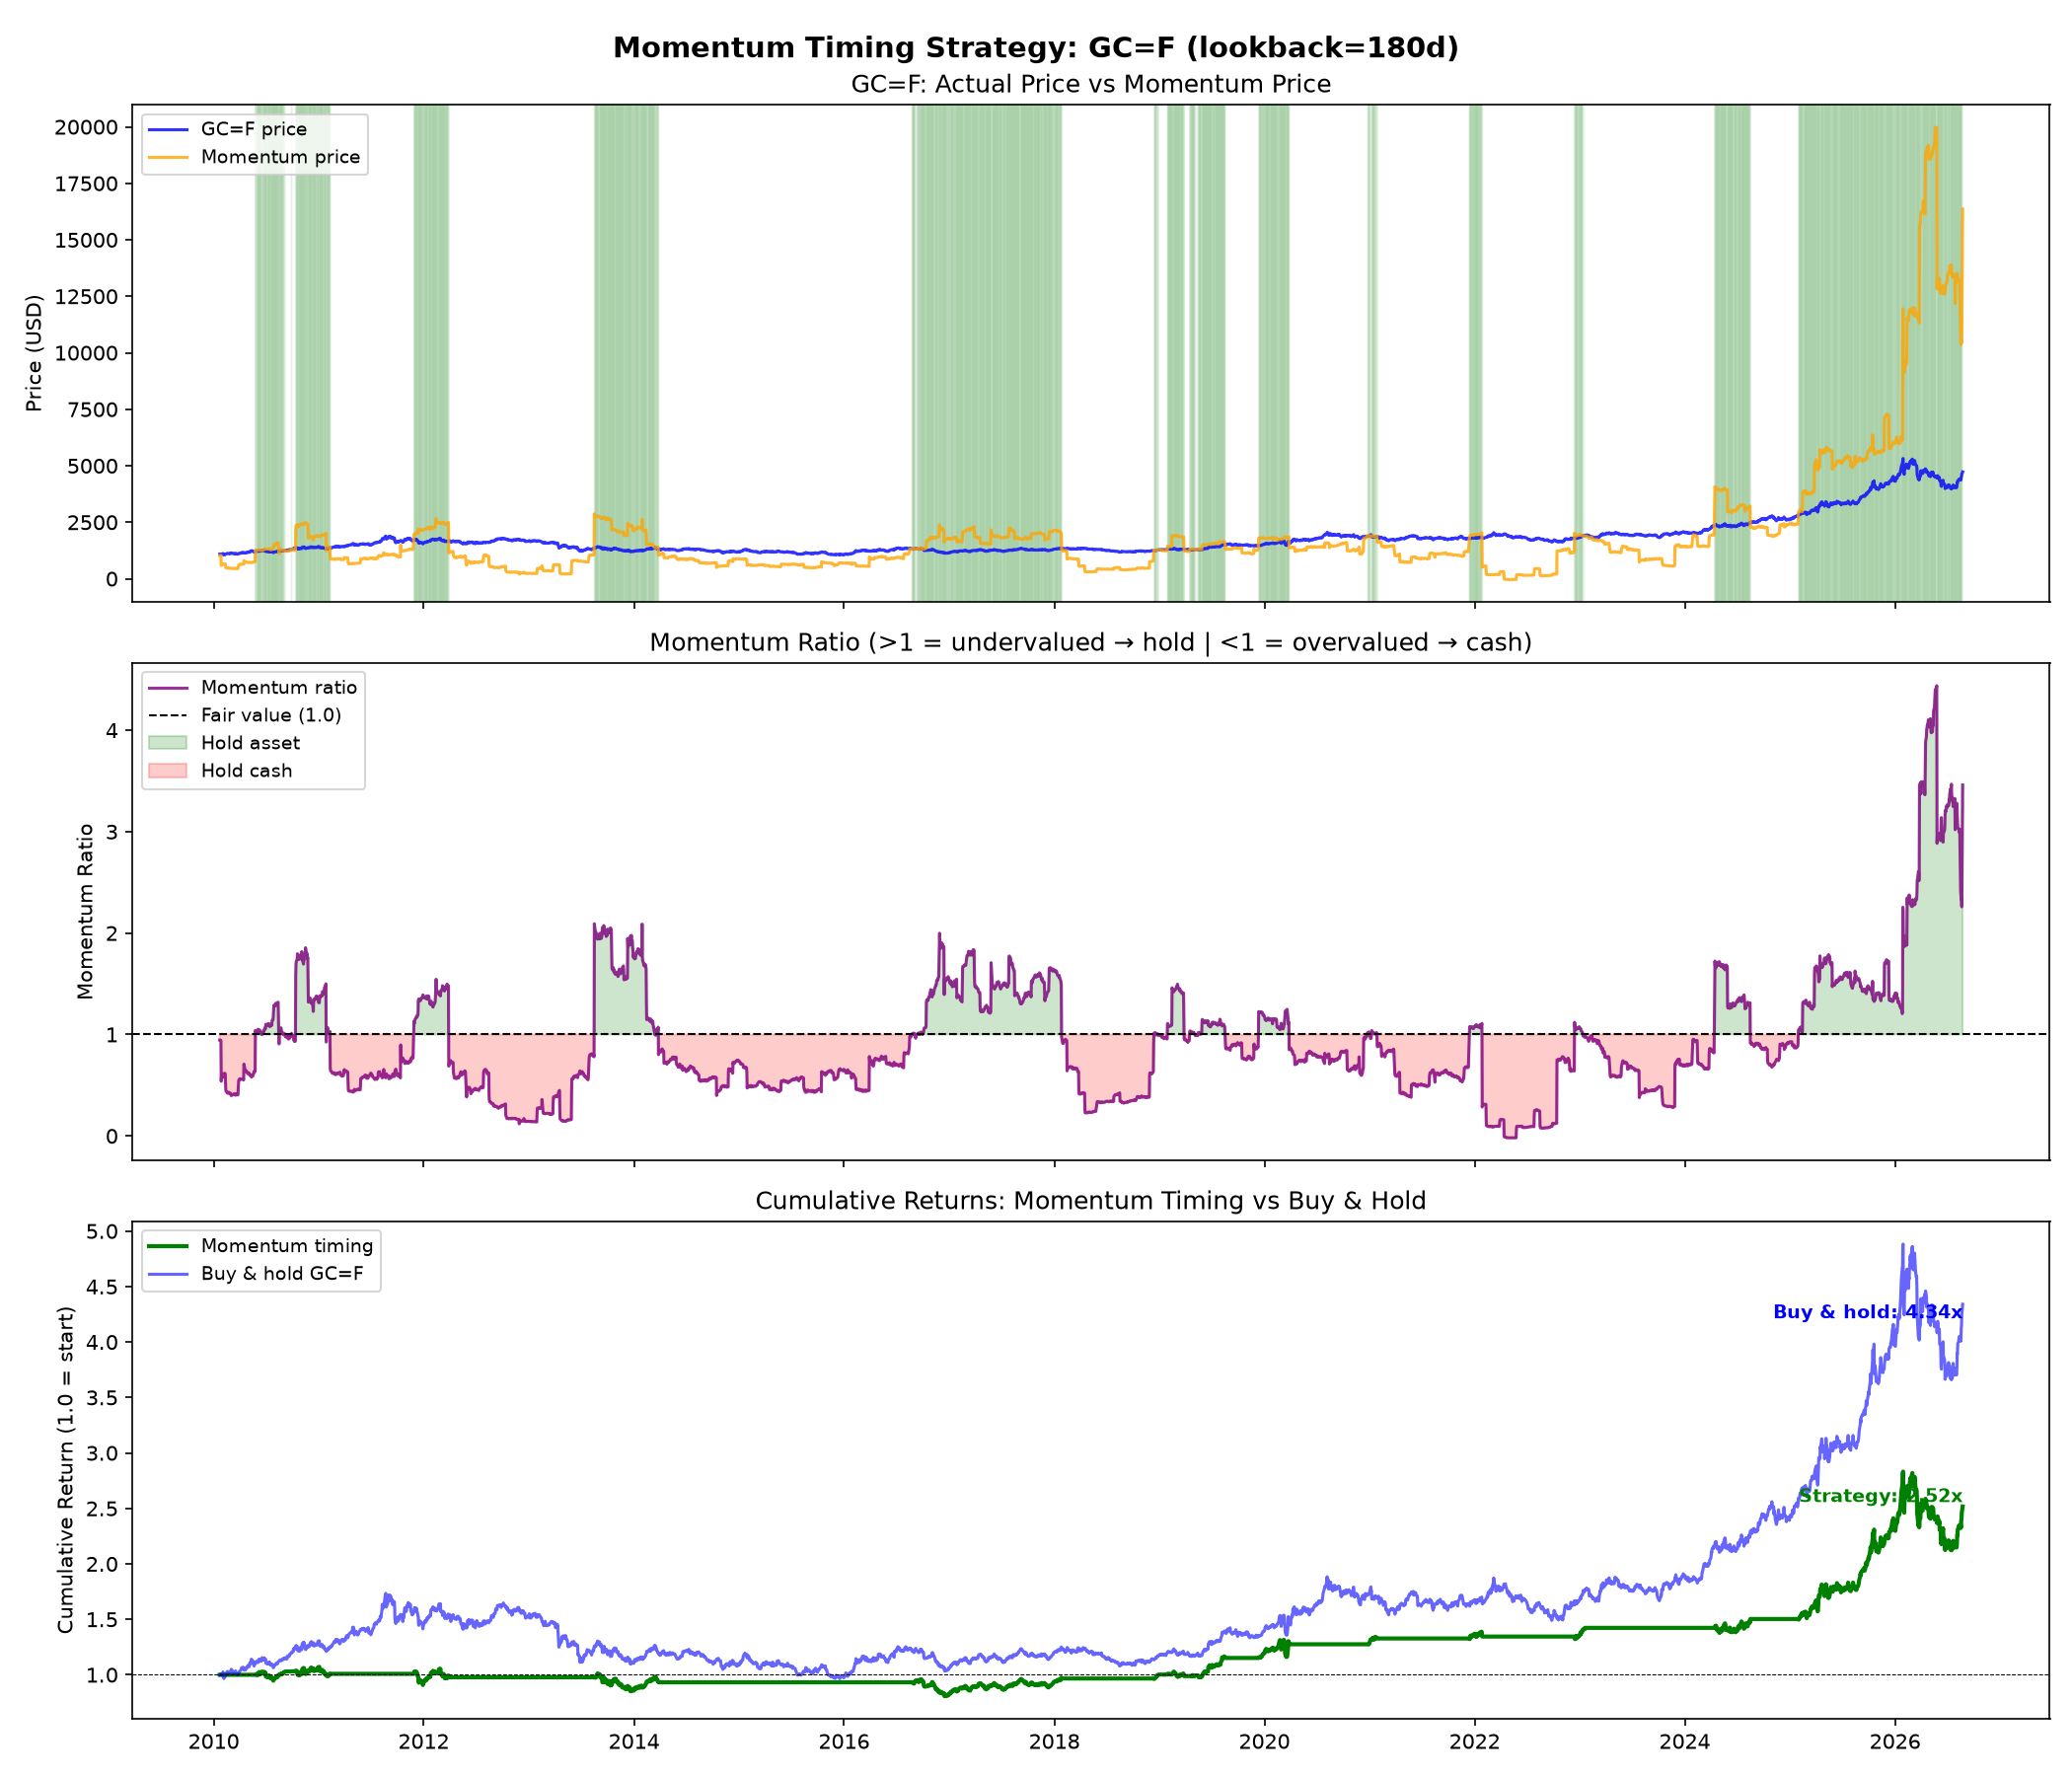
\includegraphics[width=\textwidth]{timing_gold.png}
    \caption{Gold: Actual Price vs Momentum Price (top), Momentum
    Ratio with hold/cash zones (middle), and Cumulative Returns
    (bottom). 180-day lookback, 2010--2026.}
\end{figure}

\subsection{What the Chart Shows}

\begin{enumerate}[leftmargin=2em]
    \item \textbf{2010--2011 gold bull run}: The strategy captures the
          rise from \$1,100 to \$1,900. The momentum ratio is well
          above 1.0 throughout, correctly identifying the trend.

    \item \textbf{2013 gold crash} (from \$1,700 to \$1,200): The
          strategy \textbf{partially avoids this} --- the momentum
          ratio drops below 1.0, sending the model to cash. But it
          re-enters too early and catches some of the decline.

    \item \textbf{2014--2018 dead zone}: Gold goes sideways for four
          years. The strategy oscillates in and out, generating small
          losses on each whipsaw. This is where buy \& hold pulls ahead.

    \item \textbf{2020--2026 gold surge}: Gold rises from \$1,500 to
          over \$3,000. The strategy captures much of this move, but
          misses some of the 2024--2025 rally by exiting during
          corrections.
\end{enumerate}

\subsection{Lookback Sensitivity (Gold)}

\vspace{0.5em}
\begin{tabular}{@{}lrrr@{}}
    \toprule
    \textbf{Metric} & \textbf{90-day} & \textbf{180-day} & \textbf{365-day} \\
    \midrule
    Strategy return    & $+114.5\%$ & $+151.7\%$ & $+131.6\%$ \\
    Buy \& hold return & $+323.0\%$ & $+334.1\%$ & $+316.5\%$ \\
    Alpha              & $-208.6\%$ & $-182.3\%$ & $-184.9\%$ \\
    Sharpe ratio       & $0.51$     & $0.66$     & $0.72$     \\
    Max drawdown       & $-29.3\%$  & $-25.1\%$  & $-25.1\%$  \\
    Trades             & 40         & 30         & 6          \\
    Win rate           & ---        & 60\%       & ---        \\
    \bottomrule
\end{tabular}

\vspace{0.5em}
All lookback windows underperform buy \& hold on return. The 365-day
has the best Sharpe (0.72) and lowest drawdown (-25.1\%) with only 6
trades, but still trails badly on absolute return.

\subsection{Verdict: Gold}

The strategy \textbf{does not beat buy \& hold on gold}. Why?

Gold had two massive secular rallies in this period (2010--2011 and
2020--2026), with a long sideways grind in between. The strategy
performs well \emph{during} the rallies (it correctly holds) but
gets whipsawed during the sideways years, steadily giving back
gains through small losing trades.

\textbf{What it does do well}: drawdown control. The strategy's max
drawdown is -25.1\% vs -44.4\% for buy \& hold. If your priority is
\emph{not losing money} rather than maximising return, the timing
signal has value.

%% ── SILVER ───────────────────────────────────────────────────────

\section{Silver (SI=F)}

\begin{figure}[H]
    \centering
    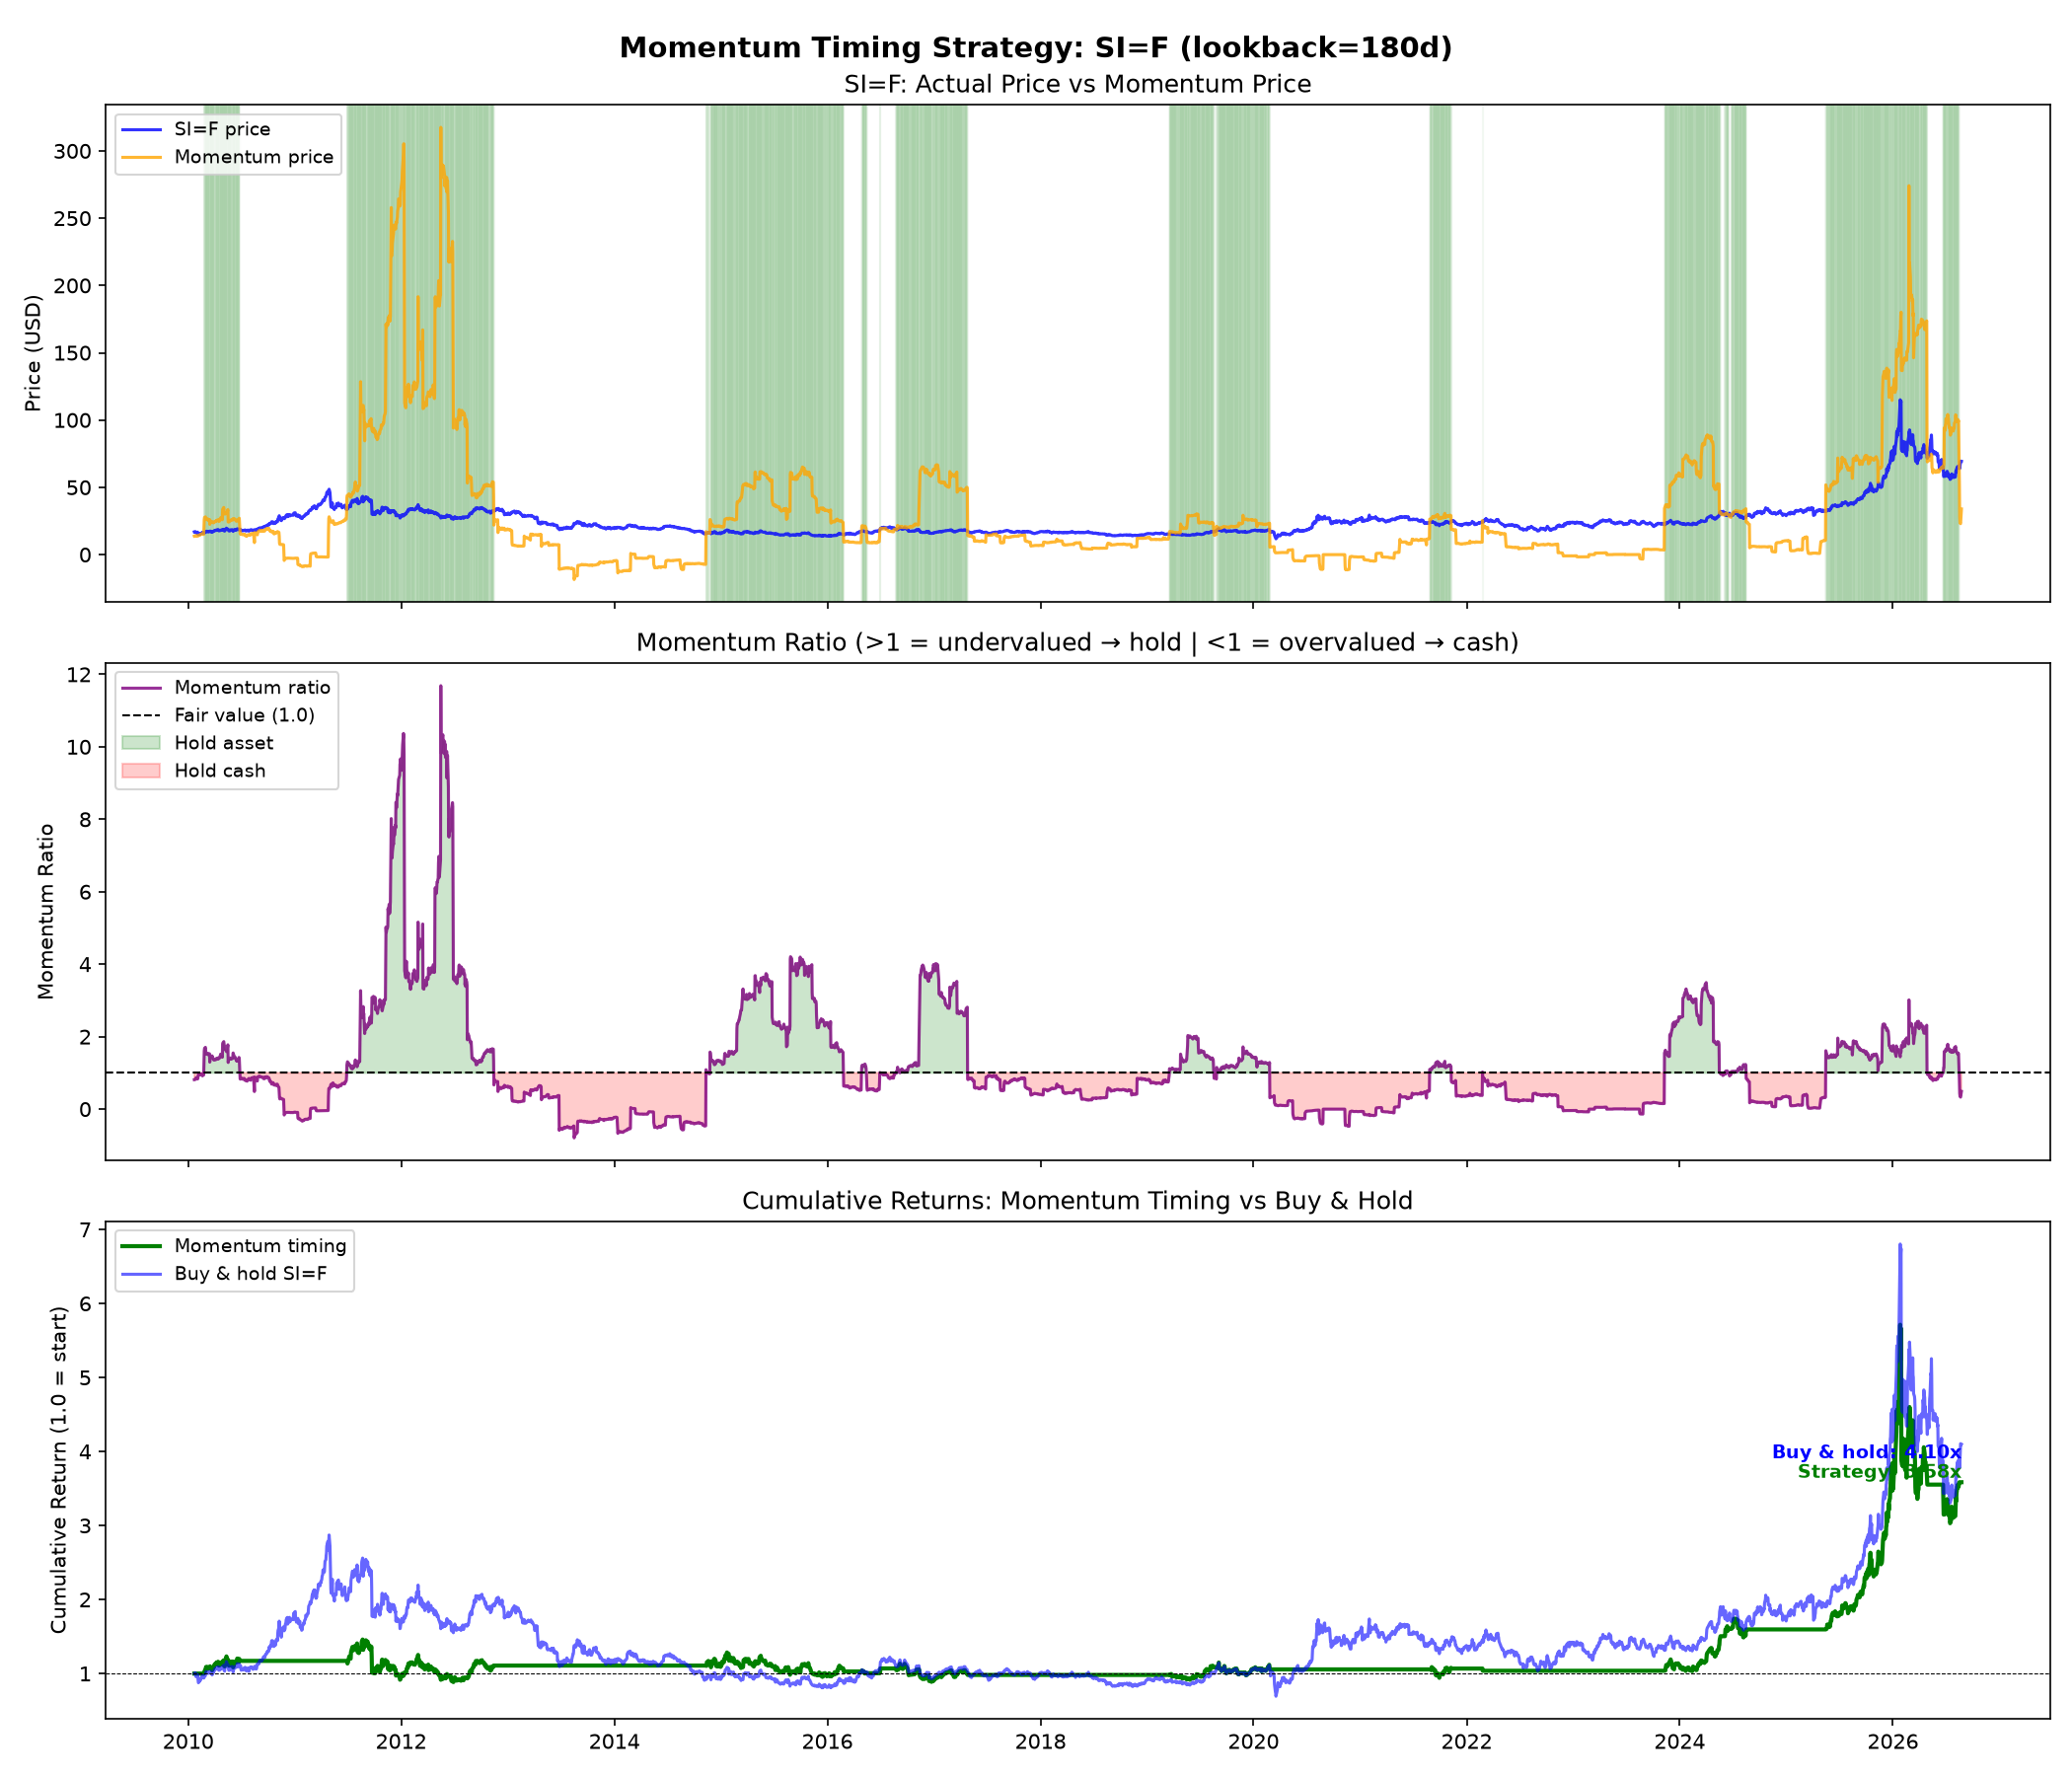
\includegraphics[width=\textwidth]{timing_silver.png}
    \caption{Silver: Actual Price vs Momentum Price (top), Momentum
    Ratio with hold/cash zones (middle), and Cumulative Returns
    (bottom). 180-day lookback, 2010--2026.}
\end{figure}

\subsection{What the Chart Shows}

\begin{enumerate}[leftmargin=2em]
    \item \textbf{2010--2011 silver spike}: Silver rocketed from \$17
          to nearly \$50 --- one of the most dramatic commodity moves
          in modern history. The strategy catches most of this, with
          the momentum ratio soaring to extreme levels (5x--10x).

    \item \textbf{2011--2015 silver crash}: Silver collapsed from \$50
          to \$14 (a -72\% decline). The strategy \textbf{exits early}
          and avoids the worst of it. This is the single most important
          event in the backtest --- it's where the strategy saves you
          from catastrophic loss.

    \item \textbf{2016--2019 consolidation}: Silver trades in a narrow
          range. The strategy mostly stays out, correctly reading the
          lack of momentum.

    \item \textbf{2020 COVID spike}: Silver surges on the Reddit/WSB
          silver squeeze narrative. The momentum ratio spikes, the
          strategy enters, and captures a large move.

    \item \textbf{2024--2026 silver rally}: Silver rises from \$22 to
          over \$50. The strategy is in for most of this.
\end{enumerate}

\subsection{Lookback Sensitivity (Silver)}

\vspace{0.5em}
\begin{tabular}{@{}lrrr@{}}
    \toprule
    \textbf{Metric} & \textbf{90-day} & \textbf{180-day} & \textbf{365-day} \\
    \midrule
    Strategy return    & $+90.0\%$  & $+258.5\%$ & $-12.5\%$  \\
    Buy \& hold return & $+297.6\%$ & $+309.9\%$ & $+291.2\%$ \\
    Alpha              & $-207.6\%$ & $-51.4\%$  & $-303.7\%$ \\
    Sharpe ratio       & $0.34$     & $0.54$     & $0.03$     \\
    Max drawdown       & $-63.9\%$  & $-46.9\%$  & $-41.0\%$  \\
    Trades             & 33         & 18         & 9          \\
    Win rate           & ---        & 67\%       & ---        \\
    \bottomrule
\end{tabular}

\vspace{0.5em}
The 180-day window is again the best performer, though the 365-day
actually \emph{loses money} ($-12.5\%$) --- far too slow to react to
silver's sharp, volatile moves.

\subsection{Verdict: Silver}

Silver is \textbf{more interesting} than gold for this strategy:

\begin{itemize}[leftmargin=2em]
    \item The 180-day strategy returns +258.5\% vs +309.9\% buy \&
          hold --- it captures \textbf{83\% of the buy \& hold return}
          while being in the market only 40\% of the time.
    \item Max drawdown is -46.9\% vs -75.8\% for buy \& hold ---
          a \textbf{massive reduction} in peak-to-trough loss.
    \item Win rate is 67\% with an asymmetry of +18.5\% avg win vs
          -5.2\% avg loss (3.6:1 ratio).
    \item It avoids 3 crashes of $>$10\%.
\end{itemize}

Silver's volatility is both a blessing and a curse. The extreme moves
(+194\% in 2010--2011, -72\% in 2011--2015) give the momentum signal
something to work with. The strategy can't beat buy \& hold on return,
but it gets you 83\% of the upside with dramatically less pain.

%% ── RECENT PERIOD ────────────────────────────────────────────────

\section{Recent Period: 2021--2026 Only}

The metals markets have changed substantially since 2020 (COVID,
inflation, central bank buying, de-dollarisation). A shorter window
may be more relevant:

\vspace{0.5em}
\begin{tabular}{@{}lrr@{}}
    \toprule
    & \textbf{Gold (5yr)} & \textbf{Silver (5yr)} \\
    \midrule
    Strategy return     & $+88.7\%$     & \textcolor{green}{\textbf{+239.3\%}} \\
    Buy \& hold return  & $+154.8\%$    & $+171.7\%$ \\
    Alpha               & $-66.2\%$     & \textcolor{green}{\textbf{+67.6\%}} \\
    Sharpe ratio        & $1.03$        & \textcolor{green}{\textbf{1.09}} \\
    Max drawdown        & $-25.1\%$     & $-46.9\%$  \\
    Win rate            & 83\% (5/6)    & 88\% (7/8) \\
    Avg win             & $+16.4\%$     & $+26.1\%$  \\
    Avg loss            & $-0.7\%$      & $-2.0\%$   \\
    \bottomrule
\end{tabular}

\vspace{0.5em}
\textbf{Silver in the recent period is the standout result.}
+239.3\% vs +171.7\% buy \& hold, \textbf{+67.6\% alpha}, Sharpe of
1.09, and an 88\% win rate with a 13:1 win/loss asymmetry
(+26.1\% vs -2.0\%).

Gold doesn't beat buy \& hold but achieves a strong Sharpe of 1.03
and an 83\% win rate with a 23:1 asymmetry (+16.4\% vs -0.7\%).

%% ── COMPARISON WITH BTC ──────────────────────────────────────────

\section{Comparison Across All Assets}

Combining results from the crypto report and this precious metals
report (all using 180-day lookback):

\vspace{0.5em}
\begin{tabular}{@{}lrrrr@{}}
    \toprule
    & \textbf{BTC} & \textbf{Gold} & \textbf{Silver} & \textbf{ETH} \\
    & \textbf{(5yr)} & \textbf{(16yr)} & \textbf{(16yr)} & \textbf{(5yr)} \\
    \midrule
    Strategy return     & \textcolor{green}{\textbf{+462.7\%}} & $+151.7\%$ & $+258.5\%$ & $+86.1\%$  \\
    Buy \& hold         & $+167.5\%$ & $+334.1\%$ & $+309.9\%$ & $+241.4\%$ \\
    Alpha               & \textcolor{green}{\textbf{+295.2\%}} & $-182.3\%$ & $-51.4\%$  & $-155.2\%$ \\
    Sharpe              & \textcolor{green}{\textbf{1.16}} & $0.66$  & $0.54$  & $0.50$  \\
    Max drawdown        & $-28.1\%$  & $-25.1\%$  & $-46.9\%$  & $-56.0\%$  \\
    Buy \& hold DD      & $-76.6\%$  & $-44.4\%$  & $-75.8\%$  & $-79.4\%$  \\
    Days in asset       & 34\%       & 36\%       & 40\%       & 26\%       \\
    Win rate            & 62\%       & 60\%       & 67\%       & 50\%       \\
    \bottomrule
\end{tabular}

\vspace{0.5em}
Observations:

\begin{enumerate}[leftmargin=2em]
    \item \textbf{BTC is the only asset with positive alpha} over its
          test period. The momentum signal is strongest where
          volatility is highest and volume most clearly reflects
          directional conviction.

    \item \textbf{All assets show drawdown reduction.} Even where the
          strategy underperforms on return, it consistently reduces
          max drawdown. The model is better at telling you
          \emph{when to get out} than \emph{when to get in}.

    \item \textbf{Time in market is remarkably consistent} --- 26--40\%
          across all assets. The model naturally keeps you in cash
          most of the time.

    \item \textbf{Win/loss asymmetry is universal.} Average wins are
          always much larger than average losses. The model cuts
          losers fast and lets winners run.

    \item \textbf{Gold is the safest application.} Lowest max
          drawdown (-25.1\%), highest win/loss ratio in the recent
          period (23:1). You give up return but sleep well at night.

    \item \textbf{Silver in the recent period} (2021--2026) is the
          only precious metal with positive alpha (+67.6\%), suggesting
          the model may work better in the current inflationary regime.
\end{enumerate}

%% ── CONCLUSION ───────────────────────────────────────────────────

\section{Conclusion}

The bookmaker pool model, applied to precious metals:

\begin{itemize}[leftmargin=2em]
    \item \textbf{Does not generate alpha on gold over 16 years.}
          Gold's long sideways periods create whipsaw losses that eat
          the gains from catching rallies. However, it dramatically
          reduces drawdown and achieves an 83\% win rate in the recent
          period.

    \item \textbf{Shows promise on silver.} Over 16 years, it captures
          83\% of buy \& hold return with far less drawdown. In the
          recent period (2021--2026), it generates \textbf{+67.6\% alpha}
          with a Sharpe of 1.09 and 88\% win rate.

    \item \textbf{Confirms the 180-day lookback} as the optimal window
          across all asset classes tested (ASX equities, BTC, gold,
          silver). This is now a robust finding.

    \item \textbf{The model's real strength is risk management}, not
          return generation. Across every asset tested, it reduces max
          drawdown substantially while keeping you in the market only
          a third of the time.
\end{itemize}

If you had to pick one trade from all the results across both reports,
it would be: \textbf{BTC with 180-day momentum timing}. If you wanted
a second, more conservative position: \textbf{silver with 180-day
momentum timing}.

\vspace{2em}
\begin{center}
\textit{--- Robin}
\end{center}

\end{document}
